% !TeX root = ../main.tex
\subsection{作図について}
    作図はそもそも次の\fitblank[3]{}種類しかない.それを,問題の意図に合わせて適切に選択し,組み合わせることで,様々な問題を解くことができる.

    \begin{definitionbox}{\textbf{作図の種類}}
        \label{def:作図の種類}
        \begin{enumerate}
            \item \fitblankbf[垂直二等分線]{12}
            \item \fitblankbf[角の二等分線]{12}
            \item \fitblankbf[垂線]{12}
        \end{enumerate}
    \end{definitionbox}
\vspace{1em}

    次に,それぞれの作図の仕方を確認する前に,\textbf{線}とは何か.その正体を明かしておこう.

    それは,\fitblankbf[条件を満たす点の集合]{},すなわち\textbf{軌跡$^{*}$}である.

    それを踏まえた上で, Definition\ref{def:作図の種類}の作図におけるそれぞれの\textbf{線}の意味を確認しておこう.
\vspace{1em}

    \begin{theorembox}{\textbf{垂直二等分線の意味}}
        \label{thm:垂直二等分線の意味}
        垂直二等分線は,\fitblankbf[2点間の距離が等しい]{}点の集合である.
    \end{theorembox}
\vspace{-1.5em}

    \begin{example}[【例題 1】]
        下の図において,線分 $\mathrm{AB}$ の\textbf{垂直二等分線}を作図しなさい.
    \end{example}

    \begin{proof}\mbox{}\\
        \\
        \\
        \begin{center}
            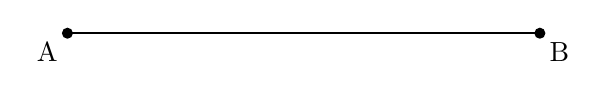
\begin{tikzpicture}[scale=1.0]
                \coordinate (A) at (0,0);
                \coordinate (B) at (6,0);
                \fill (A) circle (2pt) node[below left] {$\mathrm{A}$};
                \fill (B) circle (2pt) node[below right] {$\mathrm{B}$};
                \draw[thick] (A) -- (B);
            \end{tikzpicture}
        \end{center}
        \vspace{2em}
    \end{proof}

    \vfill
    \noindent\rule{\textwidth}{0.4pt}

    \noindent
    $^{*}$ 与えられた条件を満たしながら動く点が描く図形を,その条件を満たす点の \textbf{軌跡} という.

    詳しくは,数学Ⅱ「図形と方程式」で学習する.

\newpage

    \begin{theorembox}{\textbf{角の二等分線の意味}}
        \label{thm:角の二等分線の意味}
        角の二等分線は,\fitblankbf[2辺間の距離が等しい]{}点の集合である.
    \end{theorembox}
\vspace{-1.5em}

    \begin{example}[【例題 2】]
        下の図において,$\angle\mathrm{AOB}$ の\textbf{角の二等分線}を作図しなさい.
    \end{example}

    \begin{proof}\mbox{}\\
        \begin{center}
            \begin{tikzpicture}[scale=0.95]
                \coordinate (O) at (0,0);
                \coordinate (A) at (5,0);
                \coordinate (B) at (2.2,3.8);
                \fill (O) circle (2pt) node[below left] {$\mathrm{O}$};
                \fill (A) circle (2pt) node[below right] {$\mathrm{A}$};
                \fill (B) circle (2pt) node[above left] {$\mathrm{B}$};
                \draw[thick] (O) -- (A);
                \draw[thick] (O) -- (B);
            \end{tikzpicture}
        \end{center}
    \end{proof}
\vspace{2.5em}

    \begin{theorembox}{\textbf{垂線の意味}}
        \label{thm:垂線の意味}
        垂線は,任意の点から直線への\fitblankbf[最短距離]{}の点の集合である.
    \end{theorembox}
\vspace{-1.5em}

    \begin{example}[【例題 3】]
        下の図において,点 $\mathrm{P}$ を通り,直線 $\ell$ に\textbf{垂直}な直線を作図しなさい.
    \end{example}

    \begin{proof}\mbox{}\\
        \\
        \\
        \begin{center}
            \begin{tikzpicture}[scale=1.0]
                \draw[thick] (0,0) -- (6.5,0) node[right] {$\ell$};
                \fill (3.5,2.2) circle (2pt) node[right, xshift=3mm] {$\mathrm{P}$};
            \end{tikzpicture}
        \end{center}
        \vspace{2em}
    \end{proof}
